This chapter provides an overview of the \gls{acr:oqe}, 
its structure and the processes adopted for its development. 

A particular emphasis is placed on transparency, reproducibility,
community-based development and testing \parencite{pagani2014}, 
the central tenets of the development process adopted since the early stages of the project. 
%
% ..............................................................................
\section{Overview of the OpenQuake-engine}
%
The \gls{acr:oqe} is an open-source hazard and risk calculation engine 
developed by the 
\href{http://globalquakemodel.org}{\gls{acr:gem}} initiative.
%
The \gls{acr:oqe} is part of OpenQuake, a suite of open-source software packages
developed by \href{http://globalquakemodel.org}{\gls{acr:gem}} (Figure
\ref{fig:oq_platform}), which comprises the \gls{acr:oqe}, the
OpenQuake-platform and a large set of tools of which the most interesting from a
hazard perspective are the hazard modellers' toolkit (see
\href{https://github.com/GEMScienceTools/hmtk}
{https://github.com/GEMScienceTools/hmtk}).

The development of the engine - started in 2010 and currently in progress -
follows established standards adopted for the development of open-source
software such as open access of the source code though an easily accessible,
website and transparency of the development process\footnote{See for example the
    documentation available on the website of the
    \href{http://opensource.org/osr}{Open-Source Initiative for a 
more comprehensive description of the development standards commonly 
adopted within the open-source software community}}.
The engine was designed to operate on computational hardware with different properties
ranging from a simple laptop to a heterogeneous cluster of multi-core machines.
The operative system currently supported is Ubuntu Linux (additional
information on the supported version and on the installation procedure can 
be found on the GEM area on github, accessible at the following link:
\href{https://github.com/gem/oq-engine}{https://github.com/gem/oq-engine}). 
% . . . . . . . . . . . . . . . . . . . . . . . . . . . . . . . . . . . > Figure
\begin{figure}[!ht]
\centering
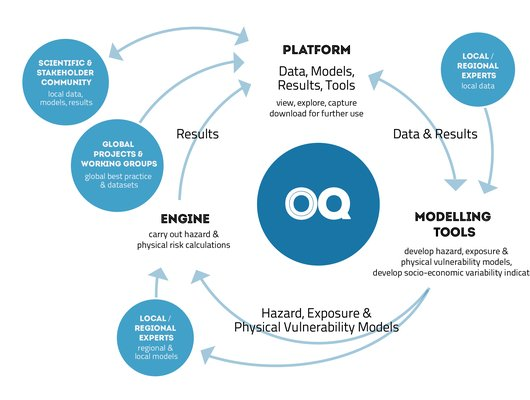
\includegraphics[width=14cm]{./Pictures/intro/OQ-workflows.jpg}
\caption{A schematic describing the OpenQuake suite.}
\label{fig:oq_platform}
\end{figure}
% . . . . . . . . . . . . . . . . . . . . . . . . . . . . . . . . . . . < Figure
%
% . . . . . . . . . . . . . . . . . . . . . . . . . . . . . . . . . . . . . . .
\subsection{Structure of the OpenQuake-engine}
The \gls{acr:oqe} is the combination of different and sometimes 
self-sufficient libraries. Below we provide a short description for each of
them.
\begin{description}
    \item [oq-hazardlib] Contains the code used to describe 
        seismic sources, create the \gls{acr:erf}, calculate hazard curves, 
        create stochastic event sets, compute ground motion fields and 
        calculate seismic hazard disaggregation.
    \item [oq-risklib] Comprises the code used to describe exposure, 
        vulnerability and fragility curves, and for the computation of losses.
    \item [oq-nrmllib] Includes the code relating to the reading, writing and validation of the full suite of \gls{acr:oqe} input and output files. The majority of these files 
        are formatted according to a dialect of 
        \href{http://www.w3.org/XML/}{XML} called \gls{acr:nrml}. 
    \item [oq-commonlib] Includes common code for \gls{acr:oqe} applications,
        such as - for example - the code used to describe logic tree structures.
    \item [oq-engine] It incorporates the core of the \gls{acr:oqe}; 
        the code in this library acts as the glue that sticks the 
        different libraries together and lets the user easily perform 
        calculations according to an established set of calculation 
        options.
\end{description}
%
% ..............................................................................
\section{Overview of the OpenQuake-engine development process}
%
The \gls{acr:oqe} is developed through a close and continuous collaboration
between the GEM scientific and IT teams. The development process is operated in
the open in order to promote the participation of experts working in the
disciplines of earthquake hazard and risk analysis, as well as those
specialising in software development.
%
% . . . . . . . . . . . . . . . . . . . . . . . . . . . . . . . . . . . . . . .
\subsection{Development tools}
%
The \gls{acr:oqe} development process is based on a number of open-source
tools, which guarantee an open and transparent process. 
%
For example, each new feature improvement or bug fix before being implemented is
described in a bug tracking system (in our case,
\href{https://launchpad.net/}{Launchpad} - see Table
\ref{tab:development_tools}). 
%
Bug tracking systems such as Launchpad keep a log of bugs and errors identified
by users of the software, in addition to requests for new features.

The tools used to maintain and make publicly available the \gls{acr:oqe}
repository and to manage the continual improvement and enhancement process are
\href{http://git-scm.com/}{git} and a git-based repository hosting service
called \href{http://github.com/}{GitHub} (see Table
\ref{tab:development_tools}). 
This process ensures comprehensive version control, facilitating the tracking of
feature implementation and bug fixing. It also ensures that previous versions of
the software can be easily retrieved.  When a developer commits new code to the
main repository the record of the change is kept. If the code is intended to
resolve a bug or error identified in the bug-tracking system, or implement a new
feature in response to a request, the log of the code contribution should
indicate the specific bug, error or feature that the code change is intended to
resolve. 
%
Thus an exhaustive and auditible record is kept of each problem
identified and the changes to the code taken to resolve it.
%
\begin{table}[!t]
\centering
\caption{Main services and websites related to the \gls{acr:oqe}}
\begin{tabular}{p{4cm}p{9cm}}
\hline
\rowcolor{anti-flashwhite}
\bf{Service} & \bf{Link}  \\
\hline 
OQ-engine main website & 
    \href{http://www.globalquakemodel.org/openquake/start/engine/}
        {http://www.globalquakemodel.org/openquake/start/engine/} \\
OQ-engine bug tracking system & 
    \href{https://launchpad.net/openquake}{https://launchpad.net/openquake} \\
OQ-engine web repository & 
    \href{http://github.com/gem}{http://github.com/gem} \\
\hline
\end{tabular}
\label{tab:development_tools}
\end{table}
Table \ref{tab:development_tools} provides a short summary of the main 
resources related to the \gls{acr:oqe}.
%
% . . . . . . . . . . . . . . . . . . . . . . . . . . . . . . . . . . . . . . .
\subsection{Programming language}
The core of the \gls{acr:oqe} is developed in 
\href{https://www.python.org/}{Python}. Python is a high-level and open-source
programming language extensively used in the scientific community 
which can run on almost all the operative systems currently available.
%
% . . . . . . . . . . . . . . . . . . . . . . . . . . . . . . . . . . . . . . .
\subsubsection{Main libraries to which the \gls{acr:oqe} depends upon}
The engine relies in on a number of open-source libraries such as:
\begin{description}
    \item [\href{http://redis.io/}{Redis}] A key-value store
    \item [\href{https://www.rabbitmq.com/}{RabbitMQ}] A messaging system
    \item [\href{http://www.celeryproject.org/}{Celery}] An asynchronous 
        task queue/job queue.
\end{description}
%
% ..............................................................................
\section{The basics of the OpenQuake-engine hazard component}
%
The hazard component of the \gls{acr:oqe} has been developed mostly following 
an object oriented programming paradigm taking, in some cases,  
concepts introduced in the development of OpenSHA, a seismic hazard 
analysis library developed within a joint SCEC-USGS collaboration 
\parencite{field2003}. 

From a conceptual point of view, the main objects adopted in the development
of the oq-hazardlib follows quite closely the classical schematic proposed by
\textcite{reiter1991} i.e. a seismic source, a ground shaking intensity model 
and a calculator that using this information computes the hazard at the site.

The \gls{acr:oqe} builds on top of oq-hazardlib and expands this 
concept by taking into account not just the essential objects 
needed to compute the hazard at a site discussed before but 
also the associated epistemic uncertainties.
%
% . . . . . . . . . . . . . . . . . . . . . . . . . . . . . . . . . . . . . . .
\subsection{Calculation workflows}
\label{sec:workflows}
% . . . . . . . . . . . . . . . . . . . . . . . . . . . . . . . . . . . > Figure
\begin{figure}[!ht]
\centering
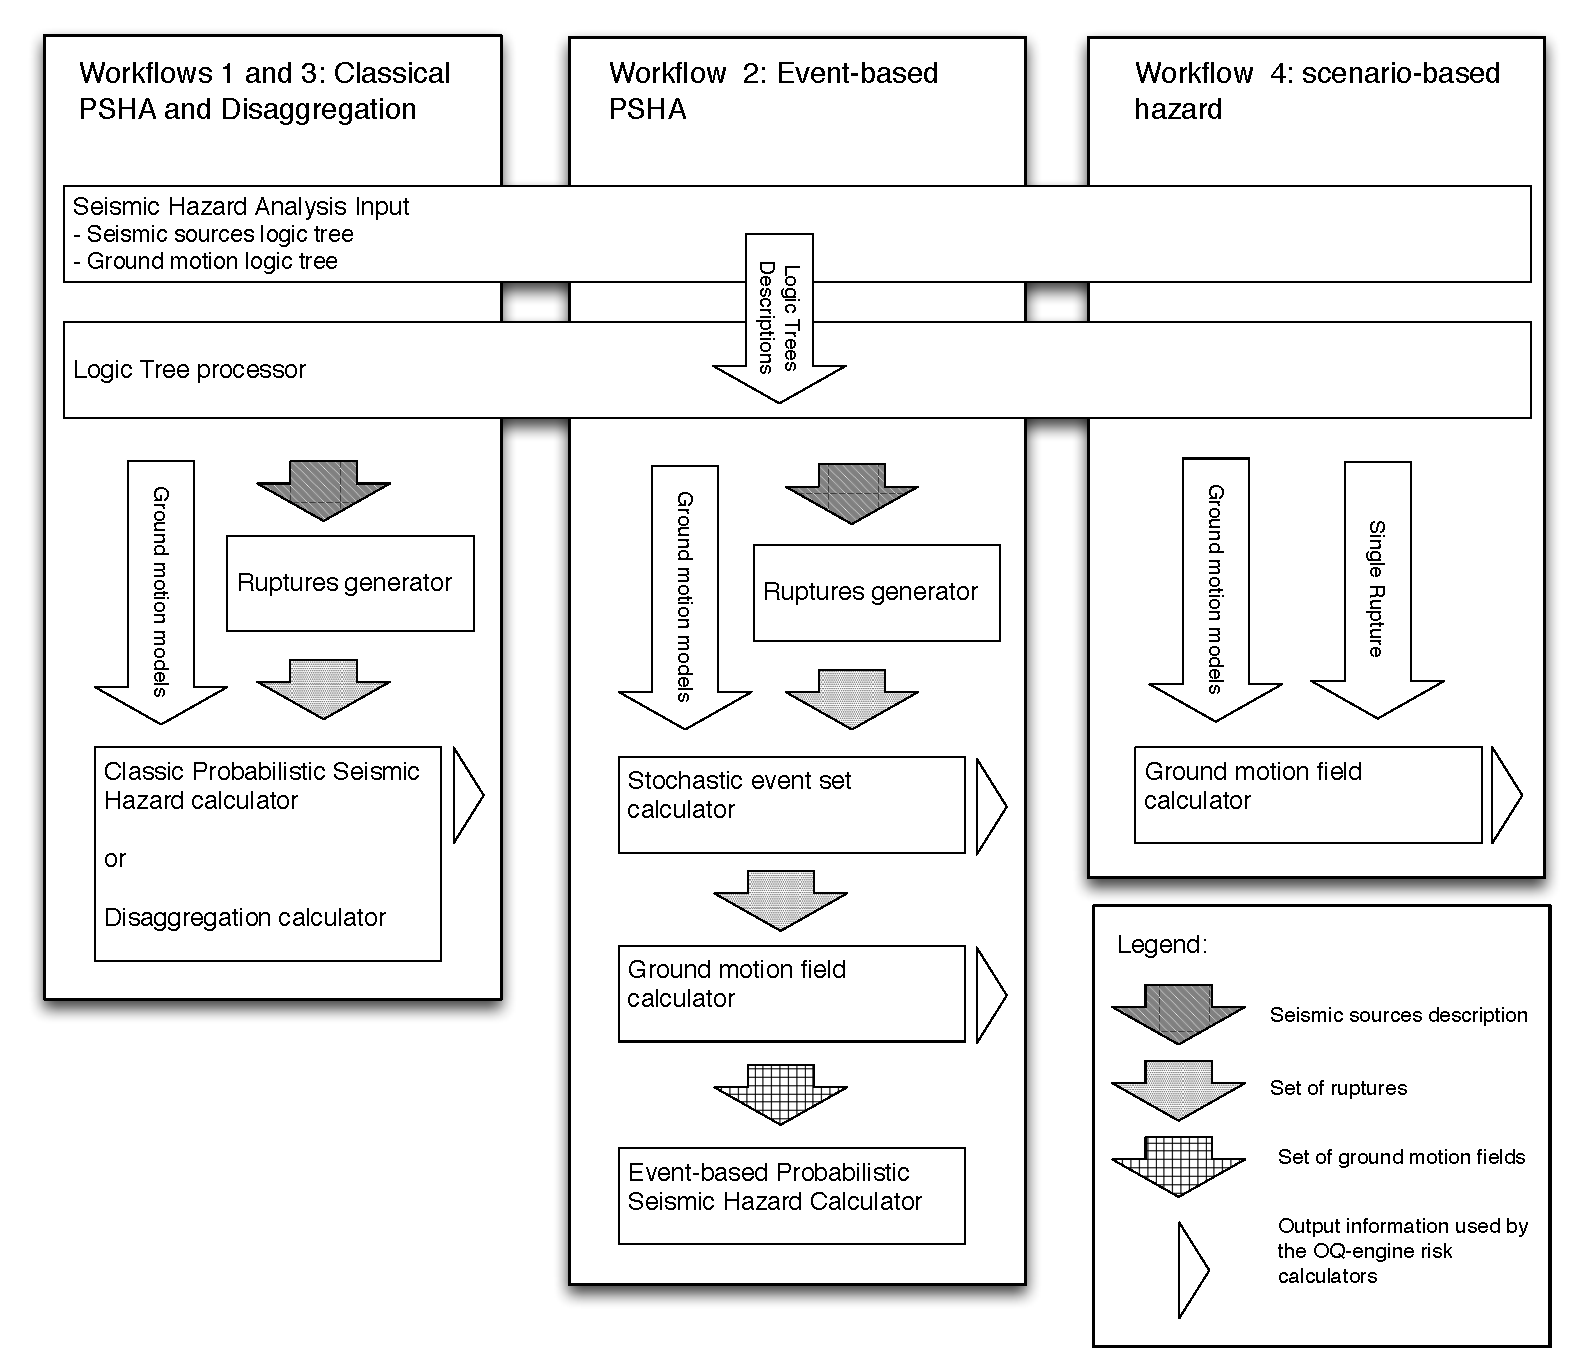
\includegraphics[width=14cm]{./Pictures/intro/fig02.pdf}
\caption{A schematic describing the main OpenQuake-engine calculation workflows 
available in the hazard component.}
\label{fig:oq_wf}
\end{figure}
% . . . . . . . . . . . . . . . . . . . . . . . . . . . . . . . . . . . < Figure

The hazard component of the \gls{acr:oqe} provides four main calculation 
workflows (see Figure \ref{fig:oq_wf}):
\begin{itemize}
\item Classical \gls{acr:psha}. Calculates hazard curves, hazard maps, 
    and uniform hazard spectra by solving the PSHA integration procedure, 
    as proposed by \textcite{field2003}. 
    This is the usual approach adopted in regional/national-scale hazard 
    assessment, as well as in site-specific studies. Using the risk 
    component of the OQ-engine, the computed hazard curves can be 
    combined with a vulnerability and exposure model to derive 
    asset-specific loss exceedance curves and loss maps for various 
    return periods. Such analyses are useful for comparative risk 
    assessment between assets at different locations, or to understand
    the areas where mitigation actions should be concentrated. 
    Crowley and Bommer (2006) suggest this methodology tends to 
    overestimate losses at high return periods for portfolios of 
    structures and recommend the use of methods capable to account 
    for the spatial correlation of ground motion residuals.
\item Event-based \gls{acr:psha}. Computes stochastic event sets (i.e., 
    synthetic catalogs of earthquake ruptures) and ground-motion fields 
    for each rupture, possibly taking into account the spatial 
    correlation of within-event residuals. This is essentially a 
    Monte Carlo–based PSHA calculator \parencite{musson2000}. The computed 
    synthetic catalogs can be used for comparisons against a real 
    catalog, whereas hazard curves and hazard maps can be derived from 
    post- processing the ground-motion fields \parencite{ebel1999}. 
    Ground-motion fields are essential input for loss estimations, 
    whereby loss exceedance curves and loss maps are calculated for 
    a collection of assets by combining a vulnerability and exposure
    model with these sets of ground-motion fields. Because the spatial
    correlation of the ground-motion residuals can be taken into account
    in this calculator, the losses to each asset can be summed per 
    ground-motion field, and a total loss exceedance curve representative 
    of the whole collection of assets can be derived. These results are 
    important for deriving reliable estimates of the variance of the
    total losses.
\item Disaggregation. Given a PSHA model, it computes the earthquake
    scenarios contributing the most to a given hazard level at a specific
    site \parencite{bazzurro1999}. Currently this is done following 
    the classical PSHA methodology; this functionality will be added to 
    the event-based calculator in subsequent development phases.
\item Scenario-based \gls{acr:sha}. Given an earthquake rupture and a 
    ground-shaking model, a set of ground-motion fields can be computed. 
    This is a typical use case for urban-scale loss analysis. This set of
    ground-motion fields can be em- ployed with a fragility/vulnerability 
    model to calculate distribution of damage/losses for a collection of
    assets. Such results are of importance for emergency management planning
    and for raising societal awareness of risk.
\end{itemize}
%
% . . . . . . . . . . . . . . . . . . . . . . . . . . . . . . . . . . . . . . .
\subsection{Testing and Quality Assurance}
%
Quality Assurance is an aspect carefully and diligently considered 
in the development of the \gls{acr:oqe}. There are a several 
different reasons for the adoption of this approach.

The first and most practical one is dictated by the development 
process which involves experts from different disciplines (e.g. 
seismic hazard and information technology). 
%
In this context the use of a formal testing process is a way through which
developers confirm the compliance of the tools developed against the
requirements defined by the scientific team and it is also a process through
which it can be demonstrated that the entire code fulfills minimum quality
criteria (e.g. the code comply with the
\href{http://legacy.python.org/dev/peps/pep-0008/}{PEP 8 standard}\footnote{As
Python is a rapidly advancing language, the Python Enhancement Proposal (PEP) is
the mechanism through which new features in the language are proposed, debated
and documented. Compliance with approved PEP standards ensures correctness of
structure and implementation of code, thus providing clarity and facilitating
continual compatibility with changes to the language.}, the code before getting
into the master repository is revised by at least one one separate developer and
is clearly documented).
 
The second motivation relates to the specific goal of building a dynamic tool
(i.e. offering a large flexibility and expandability) while constantly assuring
the stability and reliability of the supported calculation workflows.

The implementation of tests is usually done in parallel with code development,
but tests are also added for example every time a bug is fixed.
%
This improves the overall robustness and reliability of the code and reduces
drastically the possibility of regressions.

The following approaches represent the four-level suite of tests applied to the
\gls{acr:oqe} and therefore provide high quality assurance standards. Further
information can be found in the \gls{acr:oqe} testing and quality assurance
report \citep{pagani2014_oqtesting} 
%
\begin{description}
    \item [Unit-testing] A testing methodology which checks discrete 
        units of code against associated control data, expected behaviors 
        and operating procedures. A special set of unit-tests are the ones
        systematically created for every \gls{acr:gsim} implemented 
        (additional information about this specific topic is available within 
        Chapter \ref{chap:gmpes})
    \item [Testing against benchmark results] The results provided by the 
        \gls{acr:oqe} are compared against benchmark results. Several of the 
        tests defined by \textcite{thomas2010} are used to check the 
        reliability and correctness of the results provided. 
    \item [Tests against provided by other PSHA codes: simple cases] 
        The result computed with the \gls{acr:oqe} for simple models (e.g. one
        area source) are compared against the results calculated using 
        independent PSHA software.
    \item [Tests against provided by other PSHA codes: national or regional 
        PSHA input models] \hfill \\ The result computed with the \gls{acr:oqe} 
        using national or regional models are compared against the 
        results calculated using independent PSHA software.
\end{description}
\todo[inline]{Here we need to provide a description consistent with the
structure of the document on testing}
%
% ..............................................................................
%\section{Input and output description}
%
%An \gls{acr:oqe} PSHA input model is organised into a number of files each one
%including a specific information subset.
%
%The main file is the configuration file which contains information on the
%principal calculation settings (e.g. names of the files containing the source
%model and ground-motion model logic trees, type of analysis, kind of results).
%
%An \gls{acr:oqe} PSHA Input model also includes a file which describe the 
%source model logic tree, at least one file describing the initial set of seismic
%sources and their properties and one file with the ground motion model logic
%tree.
%
% ..............................................................................
\section{Description of book structure}
The following chapters are organized as follows. 

The second chapter is dedicated to the description of the hazard calculation
kernels and the methodologies adopted for the implementation of the worksflows
described in Section \ref{sec:workflows} at page \pageref{sec:workflows}. 

In the third chapter we discuss the typologies of seismic sources currently
supported by the \gls{acr:oqe} to model faults and distributed seismicity.

Chapter four focuses on \gls{acr:gsim} (comprising ground-motion prediction as
well as intensity prediction models). We describe the way they are implemented
and tested, the predictor variables currently supported, the features currently
supported such as the calculation of spatially correlated ground-motion fields
and we briefly summarize possible future developments.
 
Logic trees are the subject of Chapter 5; in this part of the book we explain
the modular structure designed to flexibly describe logic tree structures in the
\gls{acr:oqe}, 
 
The last chapter outlines the result of some calculations completed using the
different calculations workflows and source typologies discussed in Chapters
\ref{chap:calculators} and \ref{chap:ssm}.
